\documentclass[conference]{IEEEtran}
%\usepackage[top=1.2in, bottom=1.5in, left=0.8in, right=0.8in]{geometry}
\usepackage{balance}
\usepackage{graphicx}
\usepackage{xcolor}
\usepackage{enumitem}

\newcommand{\todo}[1]{\qquad\textcolor{red}{TODO: #1}\PackageWarning{TODO:}{#1!}}

\hyphenation{op-tical net-works semi-conduc-tor}

\newenvironment{steps}[1]{\begin{enumerate}[label=#1 \arabic*]}{\end{enumerate}}
\makeatletter% http://tex.stackexchange.com/questions/29517/forcing-new-line-after-item-number-in-enumerate-environment/29518#29518
\def\step{%
   \@ifnextchar[ \@step{\@noitemargtrue\@step[\@itemlabel]}}
\def\@step[#1]{\item[#1]\mbox{}\\\hspace*{\dimexpr-\labelwidth-\labelsep}}
\makeatother

\usepackage{listings}
\usepackage{color}

\definecolor{dkgreen}{rgb}{0,0.6,0}
\definecolor{gray}{rgb}{0.5,0.5,0.5}
\definecolor{mauve}{rgb}{0.58,0,0.82}

\lstset{frame=tb,
  language=Java,
  aboveskip=3mm,
  belowskip=3mm,
  showstringspaces=false,
  columns=flexible,
  basicstyle={\small\ttfamily},
  numbers=none,
  numberstyle=\tiny\color{gray},
  keywordstyle=\color{blue},
  commentstyle=\color{dkgreen},
  stringstyle=\color{mauve},
  breaklines=true,
  breakatwhitespace=true,
  tabsize=1
}

\makeatletter
\setlength{\@fptop}{0pt}
\makeatother

\begin{document}
\title{Toggle Smell Detection in Google Chrome}
\author{
Md Tajmilur Rahman, Dharani Kumar, Sumir Sarkar, Omar Faruk Miah\\
Concordia University,~Montreal,~QC,~Canada
}
\maketitle

\begin{abstract}
Identifying code smell is the first step to re-factor a software system. 
In Google Chrome developers use feature toggles to control their features 
and keep developing on a single trunk. This paper investigates code smell 
caused by improper use of feature toggles in Google Chrome that we call 
as toggle smell. Using feature toggles to hide/unhide features is an old 
concept but recently being practised in many software companies. Improper 
use of toggles might cause code smell including duplicate code, dead code, 
coupling and lack of cohesion. We classified the smells caused by toggles 
in six different patterns Dead Toggles, Nested Toggles, Combinatorial (spaghetti) Toggles, 
Mix of Compile-Time and Runtime Toggles, Legacy toggles and Spread Toggles. 
We created a tool ``Toggle Smell Detector (TSD)'' as an Eclipse plug-in using Eclipse C++ Development Tooling (CDT) to identify these toggle 
smells in major modules of Google Chrome source code. We found TODO 
nested toggles smells, TODO spaghetti toggles and TODO spread toggles in ``chrome'' and ``base'' modules of Google Chrome.\\
\end{abstract}

\begin{IEEEkeywords}
Software Refactoring, Software Re-Engineering, Software Design, FeatureToggles, Code Smell, Technical Debt, Mining Repository
\end{IEEEkeywords}

\section{Introduction}
Identifying code smell is a vital task for better re-factoring. Large amount of effort could be saved if a bad smell in a software project is detected properly. Re-factoring becomes more costly when there is lack of proper development documentations. Feature oriented Model Driven Development allows us develop software system to grow up in a feature oriented way that dictates the features to be distinguishable and understandable. To develop features in an isolated way while developing on a single trunk major software companies including Google~\cite{ChromeRepidRelease}, Facebook~\cite{Rossi2014Google} and Netflix use feature toggles to enable or disable a feature from the end-user access. However, improper use of feature toggles is a bad practice~\cite{Fowler2010FeatureToggle}. Feature toggles hide feature 
related code blocks until the feature is ready to publish. Once the 
development of a feature is done and published but still the toggle is 
left in the code, the blocked code becomes a dead code which is a technical 
debt.\\

Feature toggle is a variable used in an ``\textit{if}'' statement to control the 
features under development. Source code, related to a particular feature executes 
based on the value of a toggle or the presence/absence of the toggle itself. 
We found in Google Chrome, that they are using feature toggles to manage their 
features during development or even during testing. Some feature toggles are 
being used to allow end-users flip the behaviour of certain feature of the browser.\\

They use feature toggle to manage the features during development as well as 
in testing and canary phase.

Chrome is a popular, large open source project that has been using feature toggles for more than five years and that we use as case study in this paper. 
Instead of having a single configuration file for toggles, Chrome has 
multiple “switch files” representing toggleable sets of related features. 
In Fig~\ref{fig:switch-sets} we can see few of the switch-set files 
in Chrome containing toggles for their respective modules. 
We can see switch files for features related to how content is 
displayed in Chrome (content\_switches.cc) or to testing of GPU 
(test\_switches.cc).
\begin{figure}
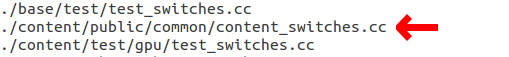
\includegraphics[height=0.5in,width=3.5in]{figure/switches.png}
\caption{Toggle set / Switch set files in Chrome source code.}
\label{fig:switch-sets}
\end{figure}
Each switch file contains a set of feature toggles that can
be enabled or disabled. In Chrome, feature toggles are strings
that can be set or unset. For example, Fig.~\ref{fig:content-toggles} 
shows that the
feature toggle kDisableFlashFullscreen3d is being set by
giving it the value “disable-flash-fullscreen-3d”. This disables
the feature that renders graphics in 3D when flash content is
presented full-screen. Advanced users might use this toggle
to improve performance~\cite{kDisableFlashFullscreen3d}.\\
\begin{figure}
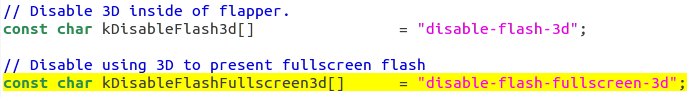
\includegraphics[height=0.5in,width=3.5in]{figure/toggleassigned.png}
\caption{Example toggles inside content\_switches.cc}
\label{fig:content-toggles}
\end{figure}

While developers are working on a feature, 
toggles are used in an if condition to let this feature
turn on/off. In Google Chrome this is done by adding a toggle 
or removing it from the switch set or feature set file. 
For the above example of kDisableFlashFullscreen3d, 
Fig.~\ref{fig:toggle-use} is showing us that the feature toggle is 
being used in an if statement and if it is set it will not allow the 
rest of the code in the function to be executed, which enables 3D 
flash-fullscreen. That means the feature 3D flash-fullscreen has been 
disabled by turning this toggle on.\\
\begin{figure}
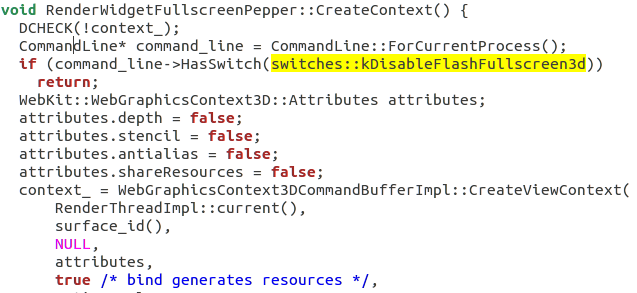
\includegraphics[height=2in,width=3.5in]{figure/toggle-use.png}
\caption{Example of use of toggle}
\label{fig:toggle-use}
\end{figure}

Commonly known code smells such as long methods, code clone, 
god class, state-checking etc.~\cite{marticorena2006extending} make the 
code hard to understand, error-prone and unmanageable for further enhancement. 
Besides the known taxonomy of code smells, toggle smells could also be joined 
in that taxonomy as considerable technical debts that need to be detected 
and re-factored for the further improvement of the software.
\\

\section{Related Works}
\label{related-works}
Continuous delivery of a software product is a recent trend in to develop software\cite{Del2006Continuous}. In order to maintain the existing features and adding or removing new features in a software system is becoming the harder thing in terms of maintains. To keep track and handle the features in some software system toggling is used. In order to study about the code smells and feature toggle, we have studied many paper but four of them most influential.\\

Jens Knoop, Oliver Ruthing, Bernhard Steffen~\cite{knoop1994partial} have worked on Partial Dead Code Elimination. They present an algorithm to eliminate partial dead code and to improve the speed of execution of program by moving the unnecessary variable assignment (Faint assignment) to the farthest location in the control flow graph, without changing the semantics of the program. The algorithm maintains a Graph whose nodes are basic block of statements and edges represents the branching information. The algorithm uses the dead code elimination techniques to eliminate the dead code and repeatedly tries to sink the assignments. In that process there are certain second order effects are classified as follows:
\textbf{Sinking - Elimination Effects},
\textbf{Sinking - Sinking Effects},
\textbf{Elimination - Sinking Effects} and \textbf{Elimination - Elimination Effects}. The algorithm addresses all the above second order effects caused by the movement of the assignment statements and also covers arbitrary control flow structures, distinguishes between the profitable code movement across the loop and fatal code movement into the loops. The dead code elimination program runs the following two functions:\textbf{dce} which eliminates the dead assignments by a dead variable analysis data and \textbf{ask} which does assignment sinking in the program by the delayability analysis.Dead variables are identified using a backward directed bit-vector based dataflow analysis technique. The dead assignments are identified using definition-use graphs.The delayability analysis is a technique to identify the location in the block of code to hoist a variable assignment.\\

Like their study we can identify the various taxonomies of toggle flag like \textbf{“INVALID TOGGLE”} and \textbf{“STABLE TOGGLE”} usages and smells  in a code base. We could leverage their techniques to see the impact of the toggle flag in the further parts of the program either in same program artifact or other artifacts so as to identify the way for their elimination. We would like to know the impacts of removing certain variable assignments (in our case toggle flags) and how it will impact the control flow structures.\\

Tiago Pessoa and his colleagues~\cite{pessoa2012eclipse} develop an Eclipse Plugin to support Code Smells using Binary Logistic Regression Model. Their tool is for detecting code smells using BLRM by using the heuristic of expert knowledge to calibrate the model. BLRM is used for estimating the probability of occurrence of an event by fitting the data set on to a logistic curve. The binary logistic regression with dependent variable having two values (either code smell present or absent) has been used to detect the probability of code smell. The BLR is calibration is done using the statistical tools like R or SPSS and JRI (Java R Inteface) is used to interface with R language from the eclipse plugin. The plugin operates in two different modes (local and remote). The plugin allows the source code to be annotated using a UI action and then collects the metrics from the annotated source code. The following metrics are calculated by the plugin for the classes and methods: \textbf{1. LOC},\textbf{2. Depth of inheritance tree},\textbf{3. Number of methods},\textbf{4. Lack of cohesion},\textbf{5. Number of parameters} and \textbf{5. McCabe Cyclomatic Complexity}\\

The authors have used binary logistic regression model in their plug-in development to determine the outcome of a code smell. We could leverage this technique to create a statistical model to determine whether there is a toggle related code smell by collecting data from the source code and using heuristic knowledge about the toggle. For example to determine whether a code block covered by a  “STABLE TOGGLE” is a potential candidate for refactoring the BLR can be trained with the meta data such as time the toggle was introduced, number of state changes during development, number of state changes in the field, number of bugs etc and the BLR can come with the prediction to indicate potential refactorings.\\

Gail C. Murphy et. al.~\cite{murphy2001separating} investigate about the separation of features in existing code.For the the purpose of the investigation they conducted an exploratory study in the context of two existing systems: \textbf{gnu.regexp and jFTPd}. They have proposed two methodologies to separate out the features from the source code which are either tangled within a single method or across several classes. In lightweight separation of concern mechanism: they discussed how far can they get by improving the object-oriented structure that exists in the system to capture features explicitly? If the feature is explicit and modularized in an object-oriented structure, then how they could use naming conventions (and other simple tools) to help decompose a feature out of a system. How the tool like Hyper/J tool could help to identify the code in an existing set of class files contributes to a particular dimension, and within a dimension to particular concerns.\\

They considered two common kinds of feature encodings in two existing Java systems. One is tangling of a feature within a method in the gnu.regexp system and another is tangling of a feature between classes in the jFTPd system.These entangling types In first case, probably lost cohesion of Lightweight SOC approach. But the splitting and restructuring was done by manually: moving fields, moving methods, forming methods, modifying inheritance and interface associations. Then they tried to separate these features using their different mechanisms (Hyper/J, AspectJ and lightweight separation of concern mechanism). Tangling in a Single Method is the method they worked with from the gnu.regexp system. This method performs part of the regular expression matching functionality. It supports several different kinds of matches, including matches across lines, matches where carat characters do not need to match at the beginning of the line and so on. Each of these kind of matches corresponds to a different feature. They wanted to separate these features that were originally tangled in a single method so as to produce a system that might support, for instance, only multi-line matches.\\

In our research objective we have to classify the code smells related to the usage of features toggles. One such code smell is to identify the distribution of the same toggles flag among various sources files, we have named this as “TOGGLE SPREAD”. This indicates the loose cohesion of a feature. This study is used to identify the features from the source code using Aspect oriented programming.\\

Pierre Genevès and Nabil Layaïda~\cite{geneves2010eliminating} studied how to detect and remove dead code from Xquery programs. They propose a technique for performing static basic dead-code analysis and eliminate the dead code from an XQuery program. XQuery is a query and functional programming language basically takes one (or possibly several) XML document as input, performs some computation based on its tree view, and finally outputs a result in the form of another XML document. The core of the XQuery language is composed of XPath expressions that make it possible to navigate in the document tree and extract nodes that satisfy some conditions. They use two methodology \textbf{Path-Error Detection} and \textbf{Static Code Refactoring and Highlighting}. In the path-error detection they gave a scema as input to an XQuery program and For each XPath expression occurring in XQuery program, they just check that it is meaningful or not with respect to the constraints described in scema. If navigational information contained in a given path contradicts the constraints described in Scema then the path will always return an empty sequence of nodes.\\

All XQuery instructions that depend on that path are dead code and maybe they should remove. For Static Code Refactoring they build an AST parser that consists in extracting all the path expressions from the program and checking their satisfiability individually. Then, in a second step, these paths are combined with the schema, and checked again for satisfiability. Each kind of unsatisfiable path is marked differently in the AST.each path is considered as a sequence of basic navigation steps possibly with qualifiers. The first step is analyzed. Then each additional step is successively appended to this initial step and the resulting path is analyzed in turn. This makes it possible to identify precisely where the error has been introduced in the path and remove them. Similarly we can detect toggle which is marked as DEAD TOGGLE in the toogle repository but still they are present in the code base but they have no impact on code flow.\\

\section{Study Setup}
\label{study-setup}
In order to explore the feature toggle related smell we have searched for open source projects and found some projects with feature toggle implemented in those project. But we have choose Google chromium as our main code base because it has more then 5 years active development life cycle with feature toggle in it and it has rapid released. So there might be any issue with feature toggle which might not notice properly. We have used Eclipse Plugin Development Environment(PDE) which is a Java based framework, it provides support for building source code analysis applications. And we have used Eclipse C++ Development Tooling (CDT) which is Eclipse variant to support development of C/C++ applications. This is where the C++ project will be loaded from google chromium source code on the test workbench.Our toggle smell detection algorithm is implemented in java. 
\section{Case Study}
\label{results}
We classified toggle smells in different classes based on their usage in 
the source code. Before that we studied different types of feature toggles 
available in Google Chrome.

\subsection{Compile Time toggles}
The first set of usage patterns we descriptively belongs to the compile 
time toggles. Here changing the toggle value requires modifying the source 
code and generating a new binary to enable or disable a particular feature 
for testing or release. The usage also relies upon the support in the 
programming language for managing enumerations. 

Even though the patterns are not complex, they are subtle for small projects (like capstone or startups) in order to manage feature dependencies and 
avoid feature branching. Another benefit of compile time toggles is, when 
cleaning up the toggle code at the end of toggle life. The location of the 
changes could be easily identified by commenting out the field containing the toggle flag.

\subsection{Constants and Variables}
In this pattern the value of the toggle state of a feature is managed through a constant variable declared in the program. In languages like C/C++, const modifiers will be used to inform that state of the feature flags will not change throughout the lifetime of the program. In Java final modifiers will be used. The data type of the variable could be a boolean or integer.\\

For example,  in Java, the constants could be declared in a final static class and used in all source files using static imports.\\

\begin{lstlisting}
public final class ToggleStates {
    public static final boolean IS_FEATURE1_ENABLED = true;
    public static final boolean IS_FEATURE2_ENABLED = true;
    ... ...
}
\end{lstlisting}

\subsection{Enumerations}
In Java there is a support to manage set of states through “enum” interface which is much richer when compared to languages like C, C++ (C++11 has similar support). The enum can implement interfaces and provide some flexibility in defining the toggle API (Togglz framework uses this approach) to use rather than using the constant variables directly.\\

\begin{lstlisting}
public enum ToggleFlags
{
    FEATURE1(false),
    FEATURE2(true),
    FEATURE3(false);

    private boolean state;
    private ToggleFlags(boolean state) { this.state = state; }

    public boolean isEnabled() { return this.state; }
}
\end{lstlisting}

The client code can directly use this \textit{enum} class method as below ``ToggleFlags.FEATURE1.isEnabled()'' which looks much cleaner in code when compared to accessing the values through constant variables.

\subsection{Compile-Time Macros}
TODO: Faruk

\section{Code Smells}
\label{discussion}

We have listed the code smells that is incurred by the usage of feature toggles on a project. We have given names that define the characteristics of the smell and provided potential causes and consequences for each smell. 

\subsection{TOGGLE\_DEAD (Dead toggles)}

\begin{table}[ht]
\caption{Dead Toggle Smell}
\centering
\begin{tabular}{|p{1.5cm}|p{7cm}|}
 \hline\hline
 Name & TOGGLE\_DEAD \\ \hline
 Description & This smell is present if the toggle repository does not possess the information about the toggle flag, but the source code is still found to use the flags to encapsulate code blocks. \\ \hline
 Example & 
 \begin{lstlisting}
if(switches::toggle1){
    Do something
}else{
    Do something else
}
 \end{lstlisting}
  \\ \hline

 Possible reasons for their presence & The possible reasons why this smell is seen in the source code are:
 \begin{enumerate}
 \item{The feature for which the toggle was added earlier became obsolete and the developers forgot to remove the toggle flag associated with the feature from the source code.}
 \item{Developer has removed the toggle flag from the toggle repository unknowingly and hence causing this smell to appear.}
 \item{There are no adequate test cases (functional/unit) to cover the code encapsulated under the toggle flag. If unit test cases were present to cover all the toggles in the toggle repository, this smell could be potentially identified by a test failure.}
 \end{enumerate}
 \\ \hline
 
 Consequences & The presence of this smell has the following consequences in the project
 \begin{enumerate}
 \item{The presence of dead code.}
 \item{If the feature is found not to be obsolete, then this smell could identify the corruption done to the toggle repository by an erroneous commit.}
 \end{enumerate}
 \\ \hline
 
Possible Detection Algorithm & This smell can be detected using the following approach:
 \begin{enumerate}
 \item{The source code will be scanned for the expressions used for detecting the state of the toggle. This could involve scanning for an invocation of a particular API or static utility method to get the current value of the toggle. An expression in this context is appropriate language syntax involved in retrieving the state of the toggle from the toggle repository.}
 \item{Typically the parameter used in this expression is the value of the toggle flag name.}
 \item{The detector will check the toggle repository for the presence of this flag.}
 \item{If the flag is absent in the toggle repository then this smell is detected.}
 \end{enumerate}
 
 \\ \hline
\end{tabular}
\label{table:chrome-dir-data}
\end{table}

\section{Our Approach}
\label{Methodology and Implimentation}
We have created a project named "tsd" which stands for toggle smell detector. This project is implemented in Java using the Eclipse Plugin development API. The solution is developed as an eclipse plugin, without user interface support. The hook to initiate the toggle smell detection is implemented using the eclipse plugin API. A toolbar button is placed in the test workbench which triggers the smell detection. This is handled through an event handler callback method which is invoked by the eclipse runtime. The solution will currently detect smells in a C++ project using the eclipse CDT API.\\

Each smell detector is implemented by a extending an abstract class which provides a skeletal implementation of the interface. The event handler callback function will invoke all the toggle smell detector classes in an order and will print the details of the detected smells in the eclipse development workbench console window.\\

Abstract syntax tree~\cite{AbstractSystaxTree} of the eclipse CDT API is utilized for each smell detection algorithm. The visitor designed pattern is applied on each of the source file to detect potential toggle smells. Each detector has an customized implementation of the AST visitor which is tailor made to detect that particular toggle smell. This design gives the flexibility to extend when an user interface is developed for this solution in the future. Typically this gives an option to detect a particular type of toggle smell in a code base by selecting the desired type from the menu. This is similar to how JDeodorant eclipse plugin user interface which has separate menu options to trigger a smell detection on a project or element within a project.

\section{Implementation Details And Algorithm}
\label{Details}
The smell detector requires following prior information to begin with:

\textbf{Toggle method signature or function name:} Without this information the toggle smell detector could not search for the pattern of the method used to check the toggle usage.

\subsection{Dead Toggle Smell Detector}
The algorithm to detect the dead and stable toggles remain the same. The detector expects a prior input from the user to provide with the list of toggle flags which became obsolete and stable. 
\begin{itemize}
  	\item The detector loads the list of stable or dead toggle flags into a mathematical Set data structure which stores string data type.
  	\item For every file, the detector checks whether it is a C++ source unit and not a header file.
  	\item For the C++ source file, an AST is constructed using the Eclipse CDT API.
	\item The AST is then traversed using a custom visitor.
	\item The visitor checks only for the conditional statements which has the toggle method function call.
	\item The parameter of the toggle method is extracted from the AST.
	\item The parameter is checked against the HashSet of strings which contain the dead or stable toggle flags.
	\item If there is a match then the particular file, line number information is captured.
	\item The locations where the dead/stable toggle flags are used in the code are stored in a data structure that is used for reporting the toggle smells.
	\item The smell detector will report the smells that are observed when all source files are scanned.
\end{itemize}
\subsection{Nested Toggle detection}
Nested toggle smell is a file level or a compilation unit level smell. The algorithm to detect the nested toggle is as follows:
\begin{itemize}
  	\item The smell detector get C++ source file from the project source roots.
  	\item For every file AST is constructed using the eclipse CDT API.
	\item An AST visitor is used to visit all the conditional branching statements (IF) for a source compilation unit.
	\item The smell detector invokes an AST visitor through the AST reference.
	\item The visitor checks only for the conditional statements which has the toggle method function call.
If there is a toggle method invocation, then the corresponding ASTNode instance is stored in a Set data structure.
	\item When a subsequent conditional statement is visited by the visitor, then the algorithm checks whether there is a parent IF conditional statement which encapsulates the current conditional statement.
	\item If there exists a parent IF conditional statement then the smell detector captures the smell information into a separate data structure.
	\item The smell detector class then consolidates all the smells from every compilation unit and store in another data structure to present for reporting the smells.
	\item The report contains information of the toggle flag which is nested under another toggle flag. The line number and file path are presented.
\end{itemize}
\subsection{(Spaghetti) Toggle Smell Detection}
Combinatorial toggle smell is a file level or a compilation unit level smell. The algorithm to detect the nested toggle is as follows:
\begin{itemize}
	\item The smell detector get C++ source file from the project source roots.
	\item For every file AST is constructed using the eclipse CDT API.
	\item An AST visitor is used to visit all the conditional branching statements (IF) for a source compilation unit.
	\item The smell detector invokes an AST visitor through the AST reference.
	\item The visitor checks only for the conditional statements which contains more than one conditional expression combined with logical AND or logical OR operators. These expressions are binary expressions.
	\item Each operand of the binary expression is compared to see whether there is a toggle method invocation.
	\item The algorithm has an recursive search function which takes the first statement and then keep searching all the expressions and extract all the arguments used in the invocation of the toggle method name.
	\item If there are more than one conditional expression within the IF statement, then a potential combinatorial toggle smell is marked by the algorithm for presenting.
	\item The smell detector class then consolidates all the smells from every compilation unit and store in another data structure to present for reporting the smells.
	\item The report contains line number of the combinatorial toggle smell in the C++ compilation unit. The line number, list of toggle flags used in that statement along with the file path are presented in the report.
\end{itemize}
\subsection{Spread Toggle Smell Detection}
The spread toggle smell is a project level smell which indicates that features are not isolated enough and might indicate high coupling in the modules.The algorithm to detect the spread toggle is as follows: 
\begin{itemize}
	\item The smell detector get C++ source file from the project source roots.
	\item For every file AST is constructed using the eclipse CDT API.
	\item An AST visitor is used to visit all the conditional branching statements (IF) for a source compilation unit.
	\item The smell detector invokes an AST visitor through the AST reference.
	\item The visitor checks only for the conditional statements which has the toggle method function call.
	\item If there is a toggle method invocation, then the method parameter is extracted and stored in a dictionary data structure with key as the parameter name and the value being the file path. The line number parameter is also recorded for reporting.
	\item Once all the source files are scanned, the detector runs through the dictionary data structure to check the toggle flags which are used in more than one file.
	\item The smell report is generated with all the toggle flags which are used in more than one file. The report includes the toggle flag name, the file and line number information where it is being used.
\end{itemize}
\section{Comparison with Alternate Solutions}
\label{comparison-with-alternate-solutions}
\subsection{Dead Toggle Detection}
There are several alternate solutions that can be used to detect the dead/stable toggle smells in the source code.

\begin{enumerate}
\item{The search for a toggle flag could be accomplished using native operating system search commands like grep or find in Linux based systems. However such search would identify all the instances of the toggle flag, for example a text based tool might give a result of finding the search item which are present in non source files, code comments etc.}

\item{Eclipse and other IDE provide search options similar to native operating system commands. This has the similar drawback as the native search tools as it might also provide search results from non source elements.}

\item{Eclipse and other IDE provide search through references and call hierarchy. This option performs the search through the internal index maintained by the IDE which is much faster than scanning each file and using the AST parser. However a developer will  have to search repeatedly for each of the dead/stable toggle flags and note down the locations of their usages and perform refactoring later.}
\end{enumerate}

\textbf{Advantages of our approach:}

Our approach to detect the toggle smells uses the abstract syntax trees from the eclipse CDT API. This makes the present solution extensible for future enhancements to suggest or perform automated or semi-automated refactorings to eliminate the dead/stable toggle from the target system.

Our solution could also be extended to do a software repository mining to identify the potential stable and dead toggle flags used in the project. The solution could then present the list of identified dead/stable toggles and present it to the developer and upon his/her confirmation could act on the detection of dead/stable toggle smells.

This way the solution does not expect manual input from the user.

\subsection{Nested Toggle detection}
To search for the presence of nested toggle smell one, a developer could use one of the following methods

\begin{enumerate}
\item{Search using native commands like find or grep. However going over the output of the grep command in order to identify the presence of nested toggle smell is very tedious and time consuming task. As the output may be large in case of a huge project code base.}
\item{The developer could also use IDE built-in capabilities to search for the instances where the toggle method is used within the source files. This gives the similar output as our smell detection algorithm, however the search does not indicate the smell, the developer has to manually introspect the source files to identify the nested toggle smell.}\\
\end{enumerate}

\textbf{Advantages of our approach: }

Presenting a solution as an plugin within an IDE like eclipse facilitates the developers to quickly navigate to the file where the smell is found. Our solution results only the places where the nested toggle smell is observed ignoring other occurrences where the toggle method name is called. So the solutions presents more narrowed down results which saves time of the developer.

As of today we are not aware of a search filter which can customize the search results such as find two or more occurrences of the invocation of the toggle method name within same class or same method. 

This search gives many instances of occurrences of the toggle method name even in the places where the nested toggle smell is not observed. So it is the developer responsibility to go over the source code to identify the nested toggle smells.

\subsection{Spread Toggle Smell Detection}

\begin{enumerate}
\item{Native OS commands:

\begin{itemize}
\item Again comparing with native operating system search commands, a user to identify a spread toggles in a huge code base involves a tedious tasks of correlating the use of toggle flag and the file names.
\item The user has to search for the existence of each toggle flag and map it with the presence in the multiple source files. That means multiple search execution for each toggle flag that he/she is interested.
\item Searching for the occurrences of the toggle method name is even difficult as the search output will be large and it will be difficult to correlate a single toggle flag spread across multiple source files from the command output.
\end{itemize}
}

\item{IDE Search:
\begin{itemize}
\item Searching for variable references or method references using IDE capabilities as found in Eclipse IDE will also involves the tedious task of correlation to the user.
\item If searched for the variable references, then again the developer has to search the code for multiple variables.
\end{itemize}
}
\end{enumerate}

\textbf{Advantages of our solution}

Our solution has an upper hand when compared with the manual searching through os commands or IDE search options might result in a large data set to correlate, compare and come to a conclusion of potential toggle smell.

Our solution presents the toggle flag name, file path and low level details like line number which saves lot of time for the developers to identify this toggle smell.

\section{Results}
\label{threats}
TODO
\subsection{Qualitative}
TODO
\subsection{Quantitative}
TODO

\section{Limitations}
\label{Limitation of our approach}
There are some limitation in our approach. The limitation are given in details according to toggles smells.
\subsection{Dead toggle}
The limitations of our approach for dead toggle are follows:

\begin{enumerate}
\item{The detector expects the input to be provided by user. This might be error prone.}
	
\item{If there is a temporary local variable used in the source file and then being used as an argument to the toggle method, then the detector will not trace the variable used and find/derive the actual value of the variable. The detector algorithm limits itself only on the token value of the argument rather than doing program analysis on the variable type and data flow.}
	
\item{The smell detector algorithm does not cross verify the toggle flag against an internal repository if any that is maintained within the target project.}
\end{enumerate}

\subsection{Nested Toggle}
The following are the limitations of the algorithm of detecting Nested Toggle:
\begin{enumerate}
\item{If there are local or member variables used within the method or the class, the algorithm will not trace the variable to find the corresponding assigned value. It will use the parameter argument from the AST. This is current implementation limitation which can be fixed to understand the semantics of the argument and identify the actual value.}
\item{Current implementation will check only for the following variants of the nested toggles

\begin{lstlisting}
IF(ToggleMethod("FLAG1")) {
	...
	IF(ToggleMethod("FLAG2") {
		…
	}
}

OR

IF(!ToggleMethod("FLAG1")) {
	…
	IF(ToggleMethod("FLAG2") {
		…
	}
}\end{lstlisting}

and the vice versa variant. It will not detect if there is a complex conditional expression if used within the conditional statement. The complex condition includes but not limited to logical AND, logical OR operators whose operands could be either the toggle method call or other expressions. 

For example the algorithm will not detect the following pattern as a nested toggle smell even though it qualifies for such smell
\begin{lstlisting}
IF(ToggleMethod("FLAG1") && ToggleMethod("FLAG2")) {
	…

	IF(ToggleMethod("FLAG3")) {
		…
	}

}	
	OR even the following pattern
	IF(ToggleMethod("FLAG1") && someVar) {
		…
		IF(ToggleMethod("FLAG3")) {
		…
	}
}
\end{lstlisting}
}
\end{enumerate}

\subsection{Combinatorial (Spaghetti) Toggle}
There is another class of spaghetti (Combinatorial) toggle code smell which involves having multiple toggle flags within a single class or single method within a class. Though this also pattern of toggle usage also qualifies for combinatorial toggle as it increases the test permutations and coverage complexity, our algorithm does not detect it at present. The implementation for the same is in progress and whose results will be published later in another publication.The following use cases are not detected by the solution: 
	1. Use of local variable or member variables of the class storing the output of the toggle method and being used in the conditional statement. As example below
\begin{lstlisting}
	bool flag1 = ToggleMethod("Flag1");
	bool flag2 = ToggleMethod("Flag2");
	bool flag3 = ToggleMethod("Flag3");

	if(flag1 && flag2 || flag3) {
		…
	}
\end{lstlisting}
	This kind of usage pattern will not be detected by the algorithm in its present form.
\subsection{Spread Toggle}
	As with limitations in the other toggle smell detection algorithms, the solution will not trace out the variables which contains the return value from the toggle method and being used in the conditional statement. 

Also use of toggle flags for other purposes without the invocation of the toggle method will not be checked by the algorithm as such usages might not indicate a potential toggle code smell.

Also many a times few configuration toggle flags will be used throughout the project, though our solution detects this usage as a toggle spread, the solution could be improved to accept feedback from the developers and should improve the search criterias.

\section{Conclusion}
\label{conclusion}
TODO

\bibliographystyle{abbrv}

\bibliography{paper}

\balance
\end{document}
